\section*{\centering PROGRAMS}
\subsection*{Unit Impilse Signal}
    \lstinputlisting[language=Octave]{code/unit_impulse.m}
    \begin{figure}[h]
        \centering
        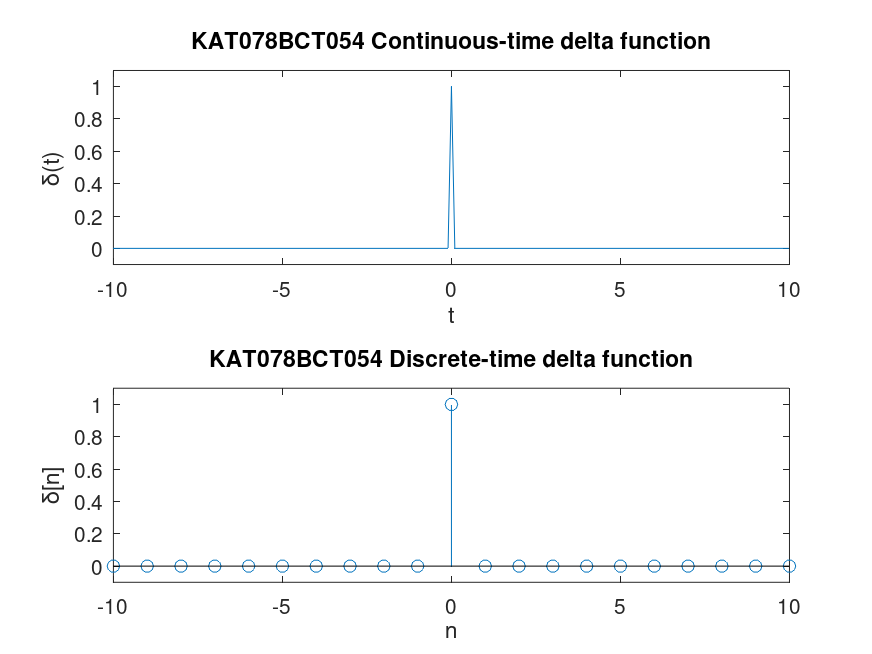
\includegraphics[width=0.7\linewidth]{figures/unit_impulse.png}
        \caption{Unit Impulse Signal}
        \label{unit_impulse}
    \end{figure}
\newpage
\subsection*{Unit Step Signal}
    \lstinputlisting[language=Octave]{code/unit_step.m}
    \begin{figure}[ht]
        \centering
        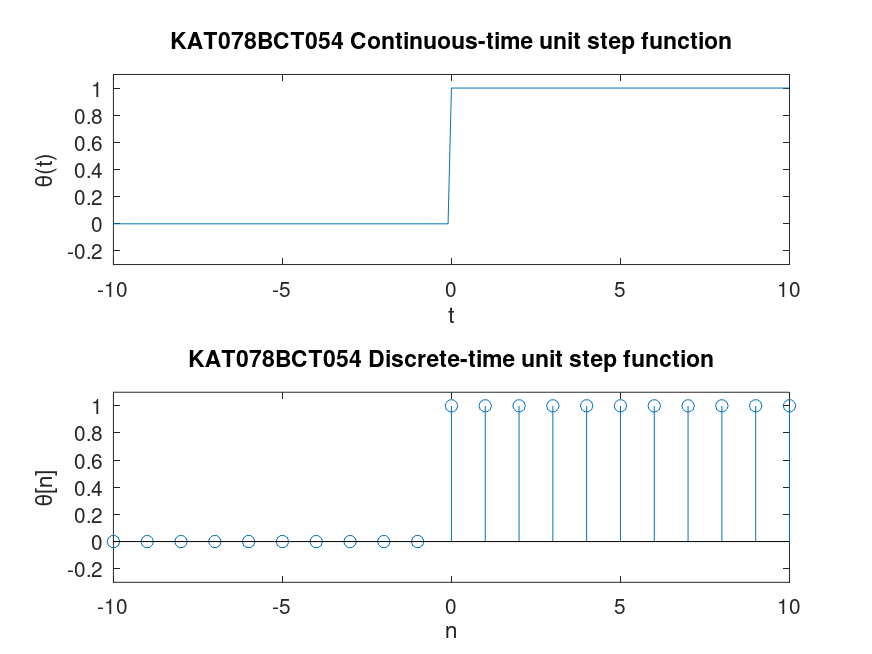
\includegraphics[width=0.7\linewidth]{figures/unit_step.png}
        \caption{Unit Step Signal}
        \label{unit_step}
    \end{figure}
\newpage
\subsection*{Ramp Signal}
    \lstinputlisting[language=Octave]{code/ramp.m}
    \begin{figure}[h]
        \centering
        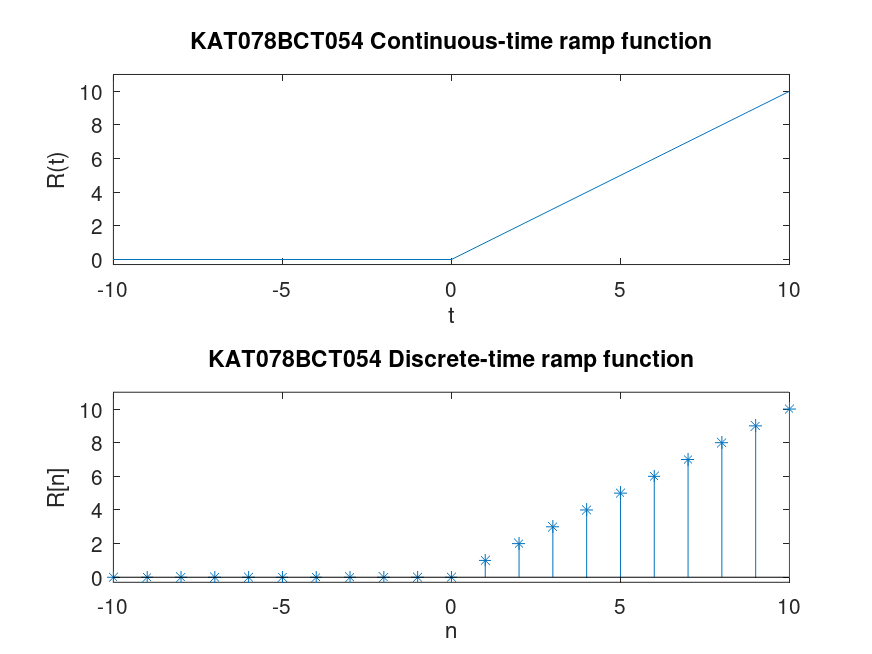
\includegraphics[width=0.7\linewidth]{figures/ramp.png}
        \caption{Ramp Signal}
        \label{ramp}
    \end{figure}
\newpage
\subsection*{Signum Signal}
    \lstinputlisting[language=Octave]{code/sgn.m}
    \begin{figure}[h]
        \centering
        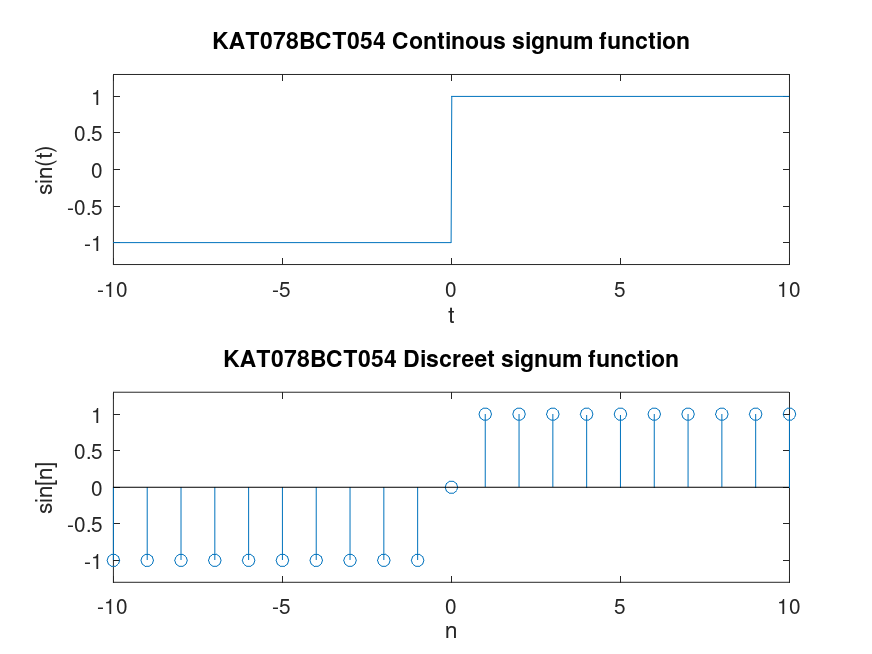
\includegraphics[width=0.7\linewidth]{figures/sgn.png}
        \caption{Signum Signal}
        \label{sgn}
    \end{figure}
\newpage
\subsection*{Rectangular Signal}
    \lstinputlisting[language=Octave]{code/rect.m}
    \begin{figure}[h]
        \centering
        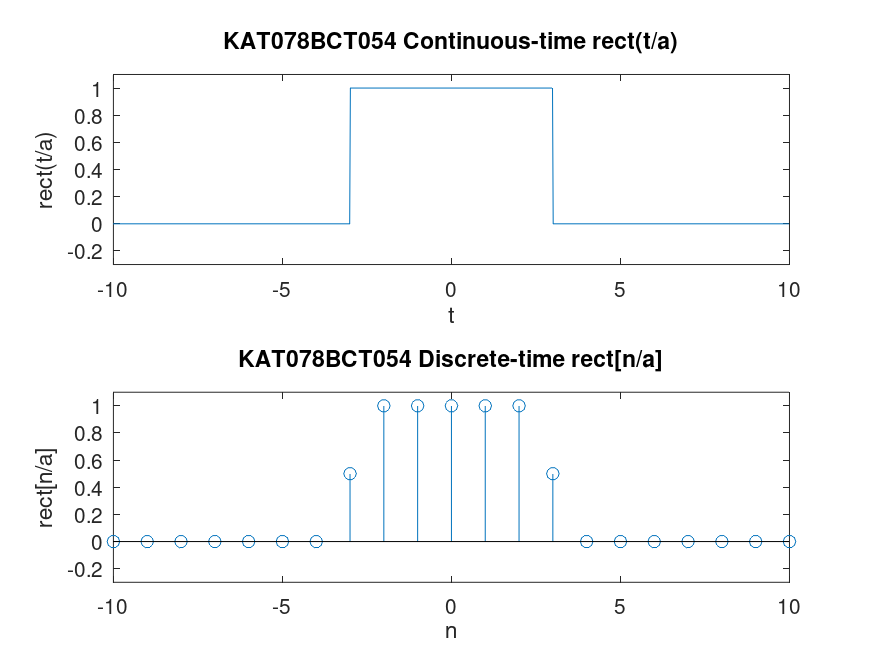
\includegraphics[width=0.6\linewidth]{figures/rect.png}
        \caption{Rectangular Signal}
        \label{rect}
    \end{figure}
\newpage
\subsection*{Sin Signal}
    \lstinputlisting[language=Octave]{code/sine.m}
    \begin{figure}[h]
        \centering
        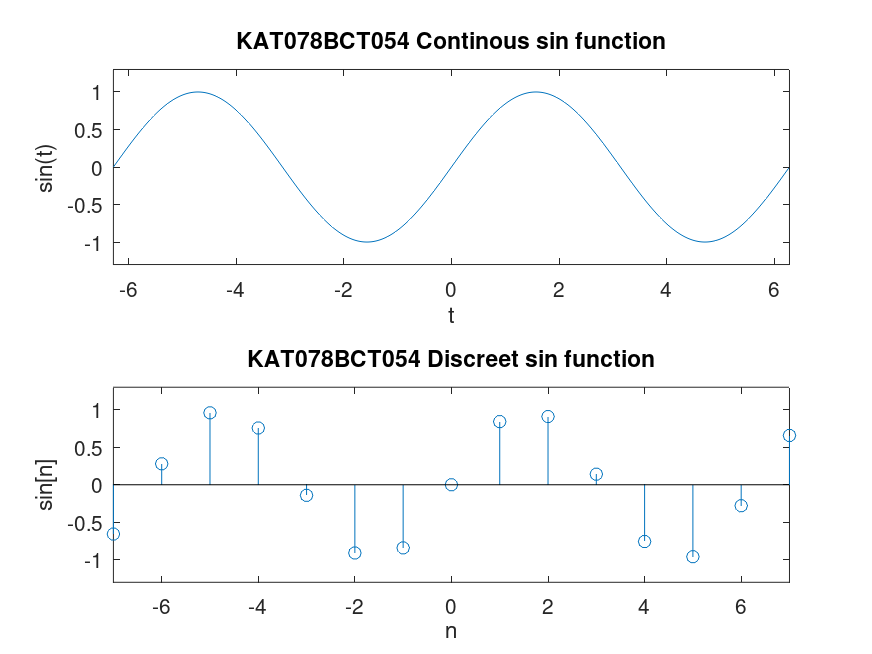
\includegraphics[width=0.7\linewidth]{figures/sin.png}
        \caption{Sin Signal}
        \label{sin}
    \end{figure}
\newpage
\subsection*{Sinc Signal}
    \lstinputlisting[language=Octave]{code/sinc.m}
    \begin{figure}[h]
        \centering
        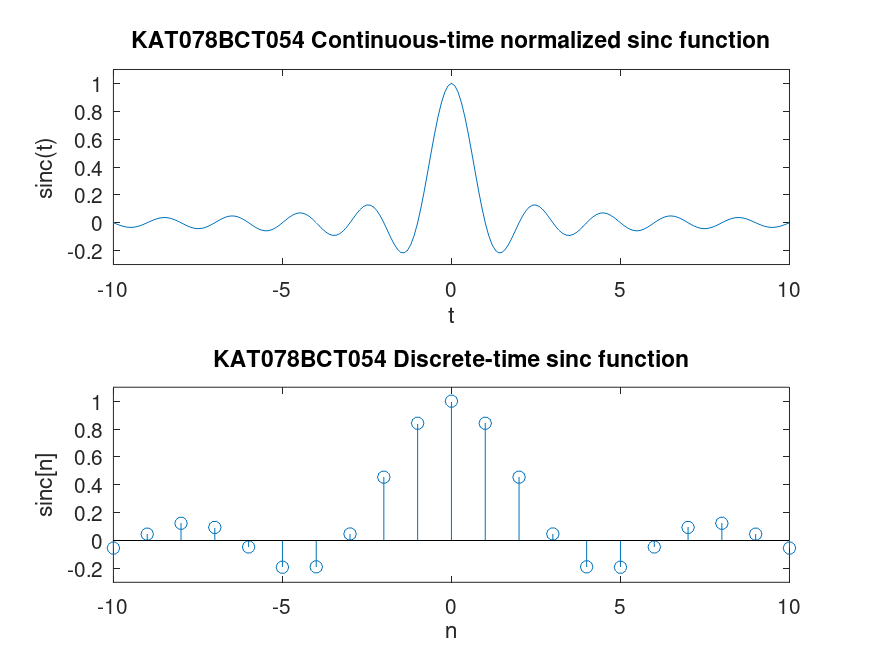
\includegraphics[width=0.7\linewidth]{figures/sinc.png}
        \caption{Sinc Signal}
        \label{sinc}
    \end{figure}
\newpage